\usetikzlibrary{shapes.geometric, arrows}

\tikzstyle{startstop} = [rectangle, rounded corners, 
minimum width=3cm, 
minimum height=1cm,
text centered, 
draw=black, 
fill=red!30]

\tikzstyle{io} = [trapezium, 
trapezium stretches=true, % A later addition
trapezium left angle=70, 
trapezium right angle=110, 
minimum width=3cm, 
minimum height=1cm, text centered, 
draw=black, fill=blue!30]

\tikzstyle{process} = [rectangle, 
minimum width=3cm, 
minimum height=1cm, 
text centered, 
text width=3cm, 
draw=black, 
fill=orange!30]

\tikzstyle{decision} = [diamond, 
minimum width=3cm, 
minimum height=1cm, 
text centered, 
draw=black, 
fill=green!30]
\tikzstyle{arrow} = [thick,->,>=stealth]

\begin{comment}
%%
% \newacronym{CAD}{CAD}{computer-aided design}
% \newacronym{PID}{PID}{proportional–integral–derivative}
% \newacronym{DNN}{DNN}{Deep Neural Network}
% \newacronym{LQR}{LQR}{linear-quadratic regulator}
% \newacronym{MPC}{MPC}{model predictive control}
% \newacronym{PD}{PD}{proportional–derivative}
%%
\end{comment}

\fancyhead[C]{Samuel Grace}

\section{Simulation and Control}
\label{sec:simcontrol}

\subsection{Introduction and Overview}

In this section of the project, software was developed to simulate the multi-agent aerial robotic system. For a drone to be able to capture useful images, it is essential that the drone can hover with minimal disturbance to its position. Achieving this stability requires a controller that is robust to sensor noise and environmental disturbances. The development of the flight control system focused on ensuring that the \gls{UAV} was sufficiently stable during a period of hovering while also making the controller suitable for general flight.

A \gls{BMS} was designed to optimise the drone's performance, further extending the mission duration as well as providing the other advantages discussed in Section \ref{sec:bms}. By combining the bespoke controller with the customised \gls{BMS} components, the performance of the \gls{UAV} was enhanced, making it ideal for detecting landmines in a wide range of environmental conditions.

The results obtained in this section were generated solely from simulations run within the C, Python, MATLAB, Simulink and Simscape environments. These simulations provided insights into the operation of the drone using a cascade \gls{PID} controller designed specifically for the chosen mission.  

Real-time environmental conditions were also modelled in the simulations. The controller is designed to be implemented onboard the drone using embedded C. The details of the hardware and software used to perform these simulations are outlined in Table \ref{tab:computersetup}. The ARM GNU Toolchain is used to test the C code developed for use onboard the drone.  
\begin{table}[h]
\vspace{5mm}
\begin{center}
\begin{tabular}{| p{6cm}|p{10cm}|}
 \hline
 \textbf{Specification}       & Details\\ 
 \hline
 Computer Model                & HP ENVY Laptop - 17-cg0002na          \\ 
 CPU Type                     & Intel Core i7-1065G7 with 4 cores, up to 3.90 GHz \\ 
 Operating System and Version & Windows 11 Home, Version 23H2, OS Build 22631.4460 \\ 
 Memory (RAM)                 & 16 GB DDR4-3200 SDRAM (2x8GB)      \\  
 Storage                      & HP 512GB PCIe NVMe M.2 SSD            \\ 
 MATLAB Version               & 24.2.0.2712019 (R2024b) \\
 Control Loop Frequency&400 Hz\\ 
  Python Version& Python 3.12.1\\
 C Version&C17 (ISO/IEC 9899:2018)\\ 
 GNU Toolchain& ARM GNU Toolchain 12.3.Rel1 (for STM32H7)\\ 
 \hline
\end{tabular}
\end{center}
\caption{Computer Hardware and Software Specifications}
\label{tab:computersetup}
\end{table}

Figure \ref{fig:simctrloverview} shows the overall scheme of the simulation and control process. First, the location coordinates were passed into the software to enable environmental, weather and climate effects to be accurately modelled. Next, the \gls{CAD} model of the drone was analysed to represent the drone's dynamics within the simulation.

An iterative simulation and refinement process was used to determine the required parameters for the cascade \gls{PID} controller used. These steps made use of the Meteomatics API to provide accurate weather data, as explained in Section \ref{gust}. Deployment of the optimised controller was then simulated in conjunction with the \gls{BMS} to ensure that the drone had adequate battery capacity for the planned mission. 

Once a single drone had been modelled, the simulation was then extended to model the multi-agent operation in the presence of motor nonidealities and environmental disturbances. The increased complexity introduced by this approach was worthwhile since it provided additional confidence that each agent could carry out their mission while maintaining a safe distance from other agents. The controller parameters could then be uploaded to the drone instantaneously; the software implementation of the cascaded \acrshort{PID} controller is fixed, allowing the loop gains to be uploaded to the microcontroller as floating-point numbers.



\begin{figure}[H]
\centering
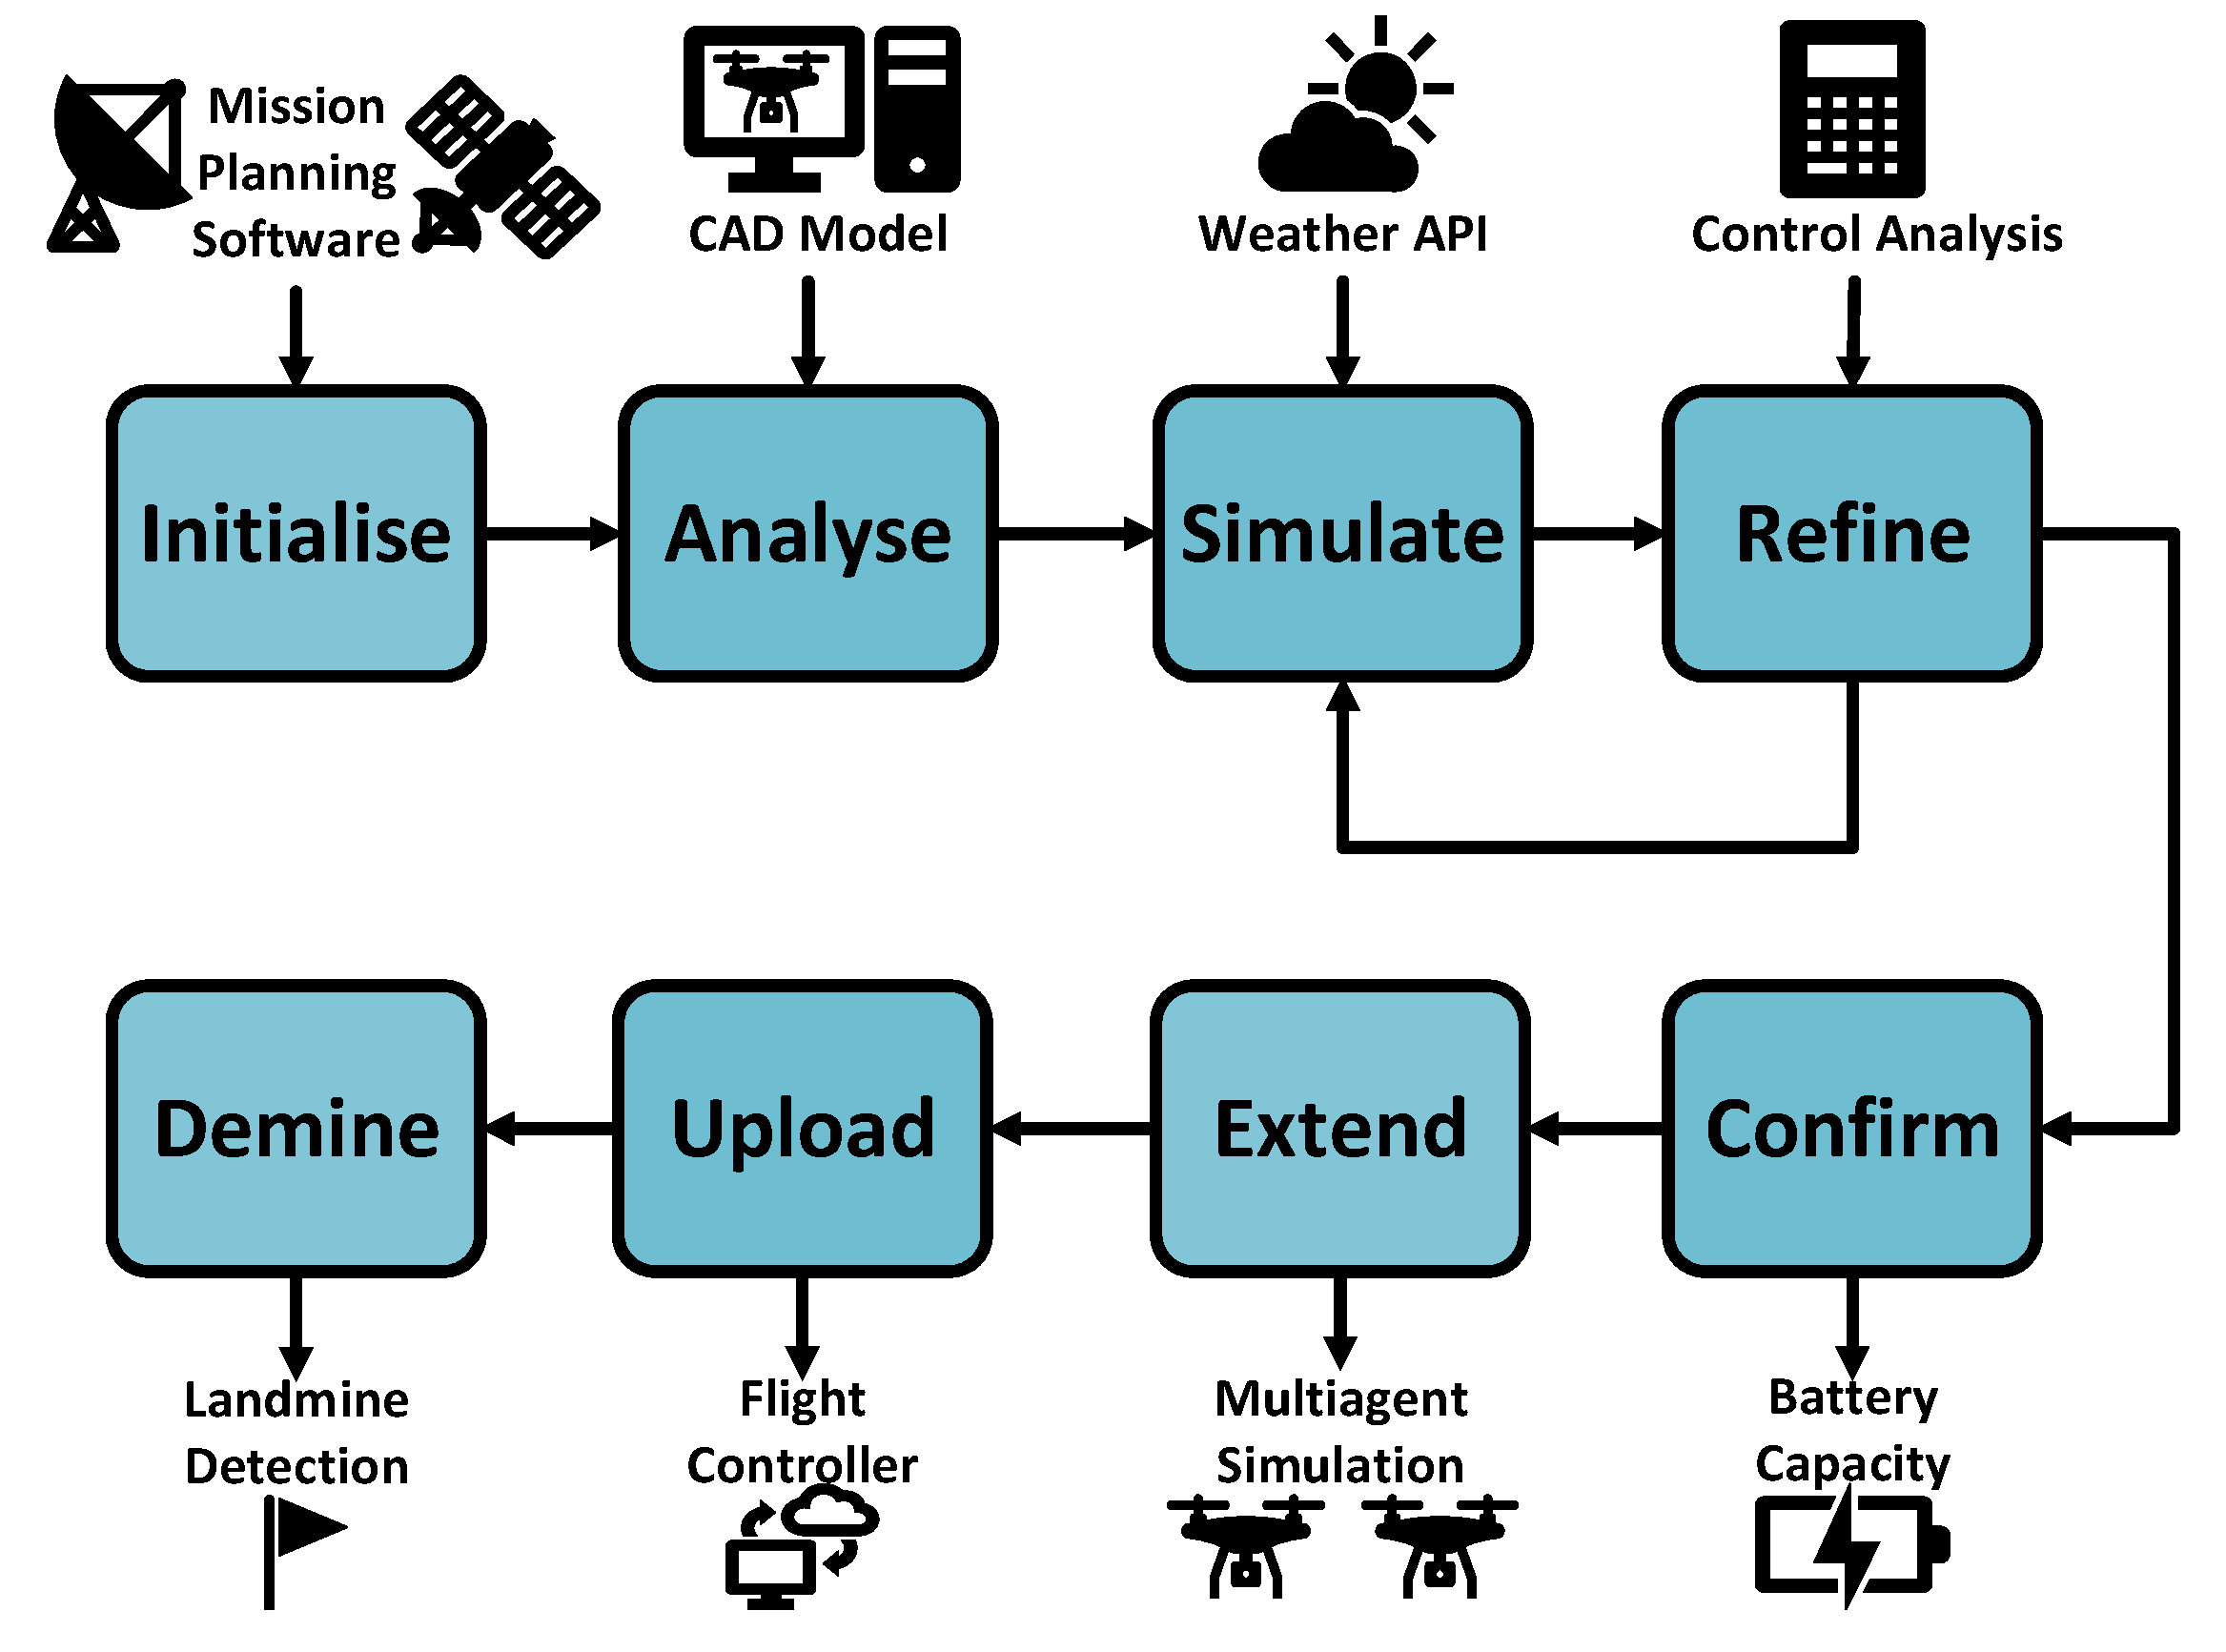
\includegraphics[width=0.87\textwidth]{figs/Samuel/Figures/Sim and Control Overview BASIC1 (1) (1).pdf}
\caption{Simulation and Control Overview}
\label{fig:simctrloverview}
\end{figure}





\subsection{Physical Modelling of the Drone Using CAD}
\label{CAD}

To simulate the drone's dynamics, it is important to have an accurate model of the drone's physical properties, including its mass, inertia tensor and the position of its centre of gravity. The drone has sensors attached, and the effects of these sensors on the drone's dynamics need to be modelled. A \textbf{Computer Aided Design (CAD)} model for the quadcopter was developed to meet these requirements. The model was rendered in SolidWorks, and an existing model was used as the basis for the quadcopter design. Figure \ref{fig:dronecad} shows the model of the drone from Westin, 2019 \cite{westin2019x4}. 

A key benefit of this approach is the ability to automatically generate the \textbf{mass properties} in SolidWorks, which includes all the necessary information for an accurate simulation of the drone. To create a drone with stable dynamics, it was essential to have symmetrically mounted components, as shown in Figure \ref{fig:2a}. The sensors and onboard processors are also centrally located to ensure that the drone can be stabilised when in the hovering position. The CAD model is also easily adaptable should there be any modifications to the drone's sensors during its operational lifetime. The drone's \textbf{inertia matrix} is shown in Figure \ref{fig:2b}, which was generated automatically.

\begin{figure}[H]
    \centering
    \begin{subfigure}[b]{0.5\textwidth} % Left-hand side: Drone image
        \centering
        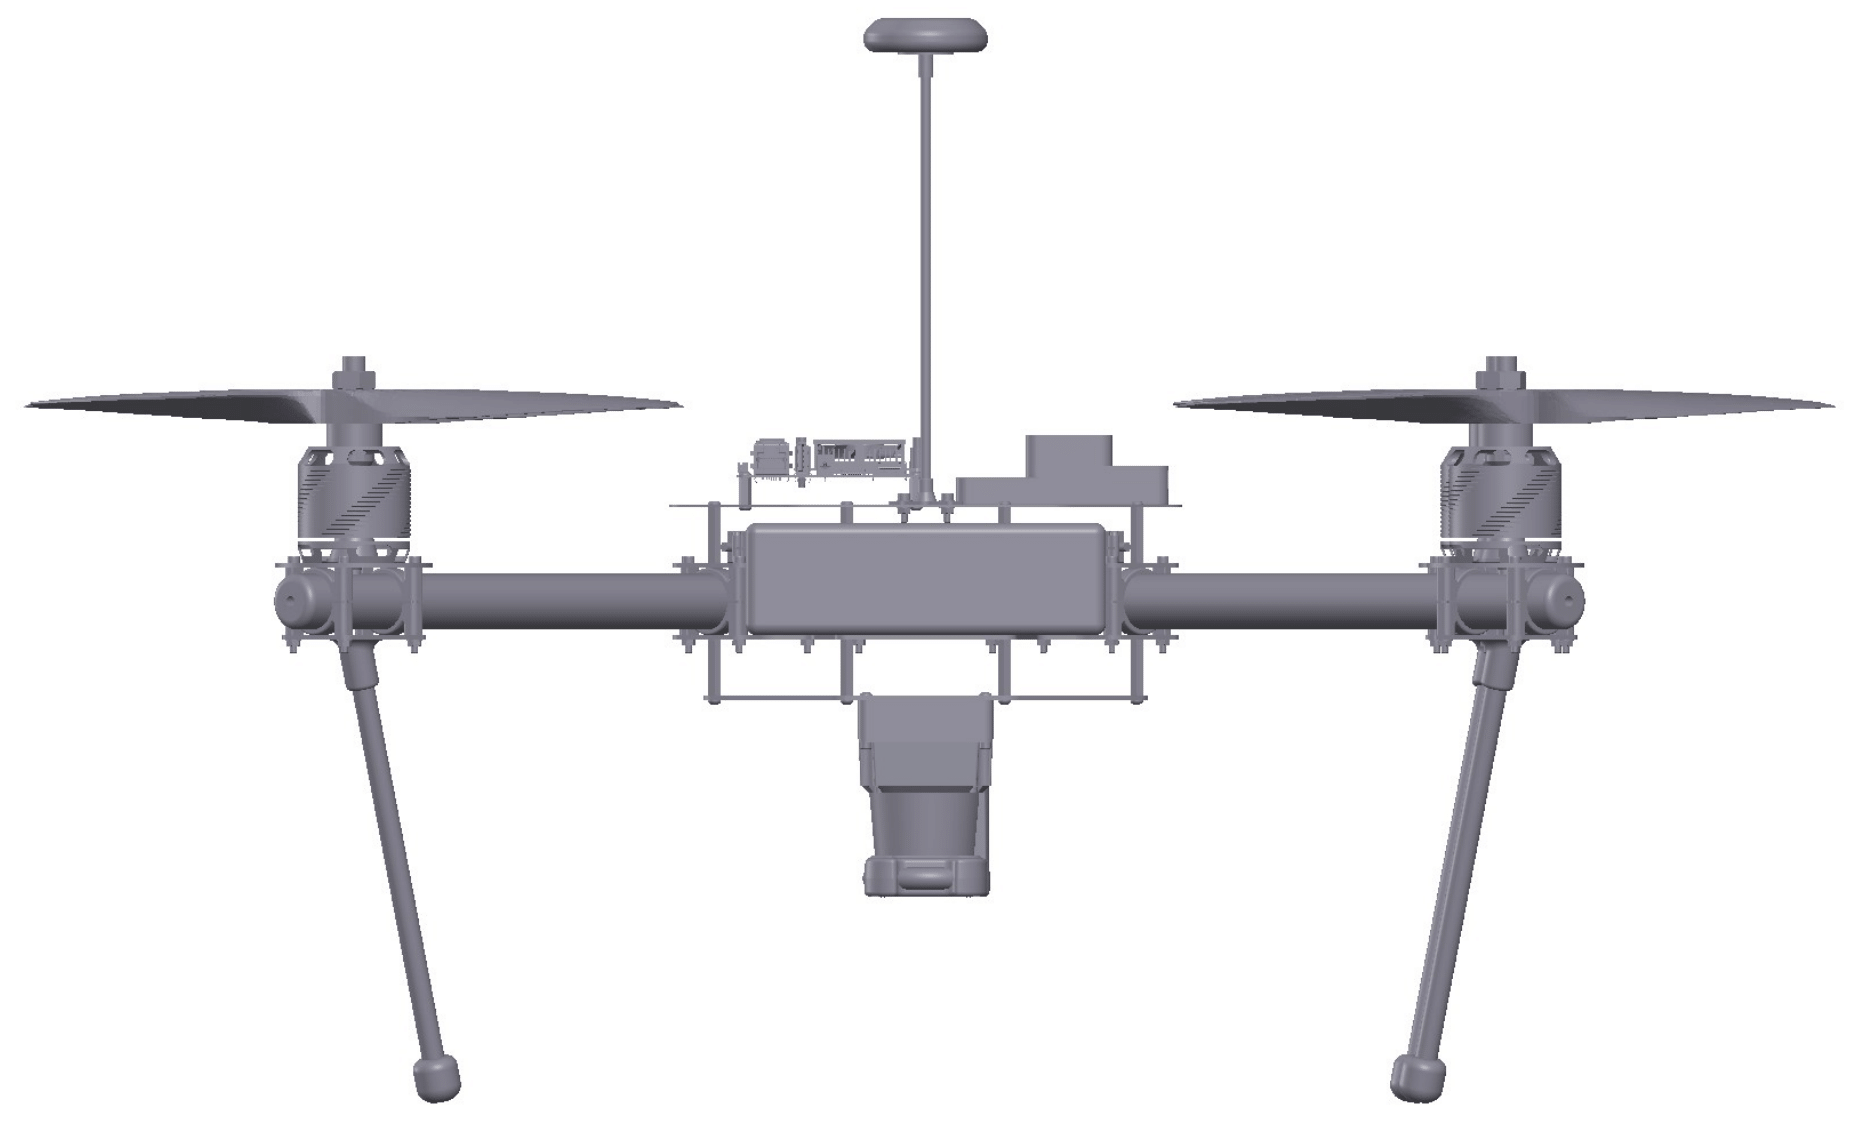
\includegraphics[width=\textwidth]{figs/Samuel/Figures/drone_new2 (cropped) (pdfresizer.com) (1)-1.png}
        \caption{Drone CAD Model}
        \label{fig:2a}
    \end{subfigure}
    \hspace{0.01\textwidth}
    \begin{subfigure}[b]{0.3\textwidth} % Right-hand side: Inertia matrix
        \centering
        \begin{equation*}
            \mathbf{I} =
            \begin{bmatrix}
                0.0875& 0.0002 & 0.0000 \\
                0.0002 & 0.0768 & 0.0185 \\
               0.0000 & 0.0185 & 0.0124
            \end{bmatrix} \quad \text{kg} \cdot \text{m}^2
        \end{equation*}
        \caption{Inertia Matrix}
        \label{fig:2b}
    \end{subfigure}
    \caption[CAD model of the UAV]{CAD model of the UAV quadcopter in SolidWorks from \cite{westin2019x4} shown in (a), with the corresponding inertia matrix shown in (b).}
    \label{fig:dronecad}
\end{figure}


\subsection{Exploration of Control Strategies}

By using the mass properties modelled in Section \ref{CAD}, it was possible to construct an accurate representation of the drone's dynamics, referred to here as the \textbf{Quadrotor Plant}. Figure \ref{fig:nekoodiag} shows the coordinate system used to model the drone, with both the \textbf{inertial frame} and \textbf{body frame} being used in the simulation. For the cascade \gls{PID} and \gls{LQR} designs, the altitude and linear velocities are taken from the inertial frame, whereas the attitude and angular velocities are taken from the body frame. The control inputs are the voltages supplied to the four rotors shown in Figure \ref{fig:nekoodiag}.


\begin{figure}[H]
\centering
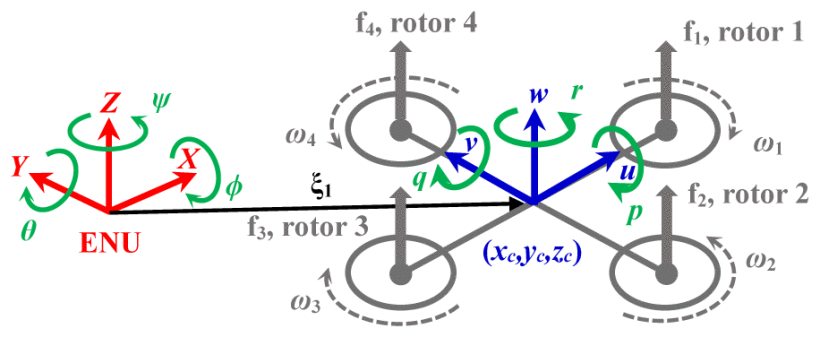
\includegraphics[width=0.66\textwidth]{figs/Samuel/Figures/nekoo1-0005-large.png}
\caption[Diagram of the drone's dynamics in inertial and body coordinates]{Diagram of the drone's dynamics in inertial and body coordinates. Source: \cite{nekoo}}
\label{fig:nekoodiag}
\end{figure}

\subsubsection{Cascade PID Control}
Since cascade \gls{PID} is ubiquitous in commercial drones, this technique was considered first. The method involves constructing nested feedback loops, with the \textbf{Attitude Controller} located inside the \textbf{Position Controller} loop. A simplified representation of the cascade \gls{PID} scheme used in the drone is shown in Figure \ref{fig:pidloop}, as in reality, the loops each have 3-dimensional states as inputs and outputs. A detailed description of the control strategy is given by \cite{electronics10040376}.

\begin{figure}[H]
\centering
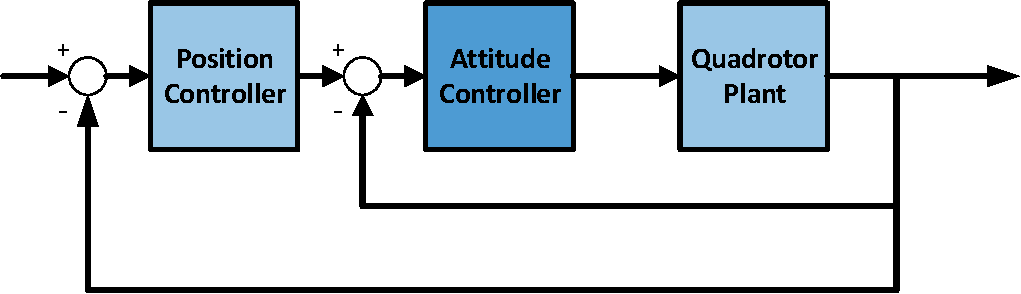
\includegraphics[width=0.79\textwidth]{figs/Samuel/Figures/Control Loop-cropped.pdf}
\caption{Cascade PID control diagram (simplified)}
\label{fig:pidloop}
\end{figure}




\subsubsection{LQR with Integral Action}
\label{sec:symbs}

In the hovering condition, position (\(x_c, y_c, z_c\)) and orientation (\(\phi, \theta, \psi\)) remain constant, with linear and angular velocities taken to be $\approx$ 0. By following the procedure outlined in \cite{cengiz2024quadcopter}, the linearised dynamics are obtained. This allows an \gls{LQR} to be constructed for the system. An LQR is an optimal state-feedback controller, computed by minimising the cost function shown in Equation \ref{eq:cost_function}:

\begin{equation} \label{eq:cost_function}
J = \int_0^\infty \left( x^\top Q x + u^\top R u \right) \, dt 
\end{equation}

$Q$ and $R$ represent the running state and input penalties, respectively. It is necessary to achieve a balance between minimising disturbances and having input demands that can reasonably be met by the actuators and battery, meaning that there is an inherent compromise between control effort and performance. Because there is no set method for selecting the state and input cost matrices, \textbf{Bryson's rule} is used to heuristically select appropriate diagonal $Q$ and $R$ matrices by setting $Q_{ii} = { [x_i]^{-2} }$ and $R_{ii} = { [u_i]^{-2} }$ where $[x_i]$ and $[u_i]$ are the states and inputs respectively \cite{chibum2014adv09designofsfb1}. The initial values are selected according to the drone's sensing capabilities and flight hardware. $Q$ and $R$ are then tuned iteratively to produce the final LQR controller design.

\subsubsection{Evaluation of Control Strategies}

Both strategies were implemented in Simulink, with the methods performing similarly in terms of overshoot and disturbance rejection. The \gls{LQR} had a slightly higher energy efficiency than the cascade \gls{PID} design, though this efficiency could be altered by adjusting the $Q$ and $R$ matrices in the \gls{LQR} design. Due to both controllers performing similarly well, computational complexity is the deciding factor. Both the implementation and tuning of a \gls{PID} controller are simpler than for an \gls{LQR} controller, so cascade \gls{PID} was selected as the control scheme.

\subsubsection{Cascade PID Analysis}
\label{sec:cascpid}

The strategy selected for implementation onboard the drone is cascade \gls{PID} control. This strategy is implemented using lightweight code on the microcontroller and can be readily optimised for any given weather conditions and mass properties. In addition, cascade \gls{PID} control is almost ubiquitous within the \gls{UAV} industry, which further suggests that it is a sensible choice. The model used for the MATLAB and Simulink simulations was modified from a cascade \gls{PD} implementation by \cite{nekoo}, by incorporating an integral term into each feedback loop. The results obtained from this simulation are shown in Figure \ref{fig:12sims}, with the symbols used defined in Section \ref{sec:symbs}. The simulation data was obtained from the case study detailed in Section \ref{mocs} and shows the drone's first 10 seconds of motion, during which it travels 10 metres in the X, Y and Z axes before settling in a constant hovering position. The disturbance of 0.4 m in the X direction during take-off is due to a gust of wind; the controller then rapidly settles to track the reference with high accuracy. The oscillation with an amplitude of 0.2 m in the Y direction is caused by the nonlinear dynamics which the simulation models, but are neglected in the \gls{PID} controller used. The dynamics in the Z-direction are less significantly affected by wind, and the output trajectory remains within 0.1 m of the reference after take-off. Around 3 seconds into the simulation, there are relatively large disturbances to the roll and pitch of up to 0.4 rad, which suggests a sudden gust of wind. The disturbance would ideally be mitigated, and is discussed further in Section \ref{gust}. The linear velocities in the X, Y and Z directions all reach between 3 and 4 ms${^{-1}}$, before decreasing towards the hovering condition of 0 ms${^{-1}}$ in all directions. The constant offset of around 0.2 ms${^{-1}}$ visible in the velocities suggests that, despite the integrator element, a non-decaying error is present in the velocity. The use of a model-free controller discussed in Section \ref{sec:modelfree} may help to alleviate this issue. Overall, the simulation produces feasible results and suggests that the model has been constructed accurately.



\begin{figure}[H]
\centering
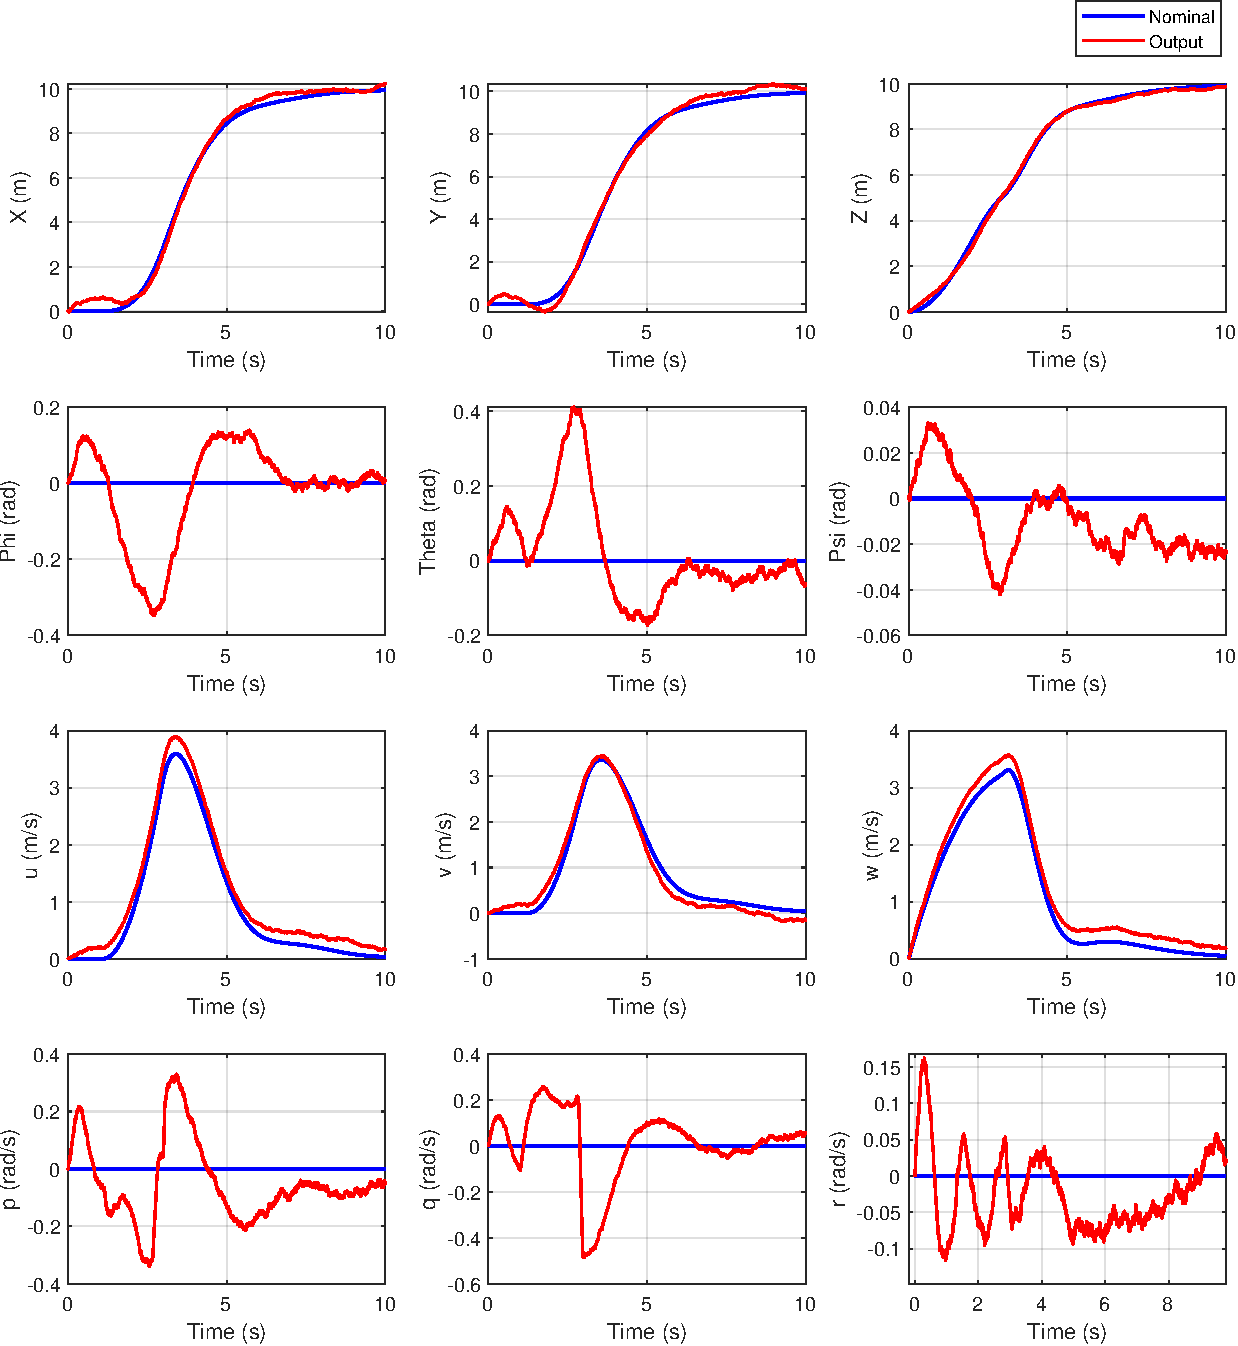
\includegraphics[width=0.75\textwidth]{figs/Samuel/Figures/twelveplotsvectorgraphic.pdf}
\caption[State Responses from the MATLAB Simulation]{State responses from the MATLAB simulation, using software adapted from \cite{nekoo}}
\label{fig:12sims}
\end{figure}










\subsection{Control Tuning Process}

To provide a bespoke controller design for each mission, the method described by the flowchart in Figure \ref{fig:drone_flow_updated} was used to iteratively update the cascade \gls{PID} loop gains until a satisfactory controller had been designed. The feedback loop ensured that the mission operator was aware of the performance capabilities of the drone; the mission duration can be varied if the environmental conditions require a controller with a higher average power consumption. The \href{https://www.meteomatics.com/}{\textbf{Meteomatics API}} provides the necessary weather data for the given location, and Section \ref{CAD} describes the model used to generate the drone's mass properties. The performance evaluation step consists of two components: the system automatically confirms that no constraints were broken and the operator manually reviews graphs of the evolution of the drone's states, as shown in Section \ref{sec:cascpid}. These two layers of verification provide additional confidence that the controller has been designed successfully. Finally, the selected loop gains are uploaded directly to the onboard microcontroller so that the cascade \gls{PID} controller can be deployed on the \gls{UAV}. 

\begin{figure}[H]
\centering
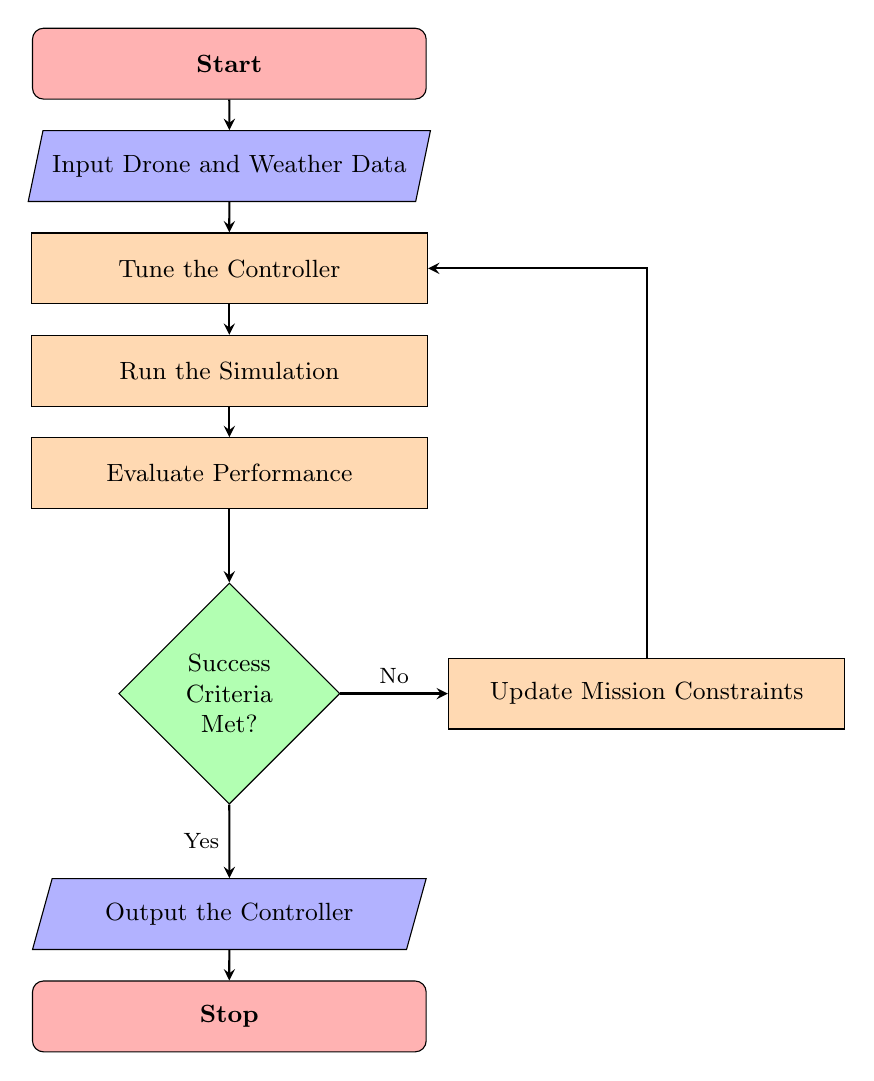
\begin{tikzpicture}[node distance=1.3cm, every node/.style={font=\small}]
% Define styles
\tikzstyle{startstop} = [rectangle, rounded corners,
minimum width=5cm,
minimum height=0.9cm,
text centered,
draw=black,
fill=red!30]

\tikzstyle{io} = [trapezium,
trapezium stretches=true,
trapezium left angle=70,
trapezium right angle=110,
minimum width=5cm,
minimum height=0.9cm,
text centered,
draw=black,
fill=blue!30]

\tikzstyle{process} = [rectangle,
minimum width=5cm,
minimum height=0.9cm,
text centered,
text width=4.8cm,
draw=black,
fill=orange!30]

\tikzstyle{decision} = [diamond,
minimum width=1.2cm,
minimum height=1.2cm,
text centered,
text width=1.35cm,
draw=black,
fill=green!30]

\tikzstyle{arrow} = [thick,->,>=stealth]

% Nodes
\node (start) [startstop] {\textbf{Start}};

\node (input) [io, below of=start, yshift=+0cm, align=center] {Input Drone and Weather Data};

\node (simulate) [process, below of=input] {Tune the Controller};

% Added "Optimize Controller" node
\node (optimize) [process, below of=simulate] {Run the Simulation};

\node (evaluate) [process, below of=optimize] {Evaluate Performance};

\node (decide) [decision, below of=evaluate, yshift=-1.5cm] {Success Criteria Met?};

\node (adjust) [process, right of=decide, xshift=4cm] {Update Mission Constraints};

\node (output) [io, below of=decide, yshift=-1.5cm, align=center] {Output the Controller};

\node (stop) [startstop, below of=output, yshift=+0cm] {\textbf{Stop}};

% Connections
\draw [arrow] (start) -- (input);
\draw [arrow] (input) -- (simulate);
\draw [arrow] (simulate) -- (optimize);
\draw [arrow] (optimize) -- (evaluate);
\draw [arrow] (evaluate) -- (decide);

\draw [arrow] (decide) -- node[anchor=east, xshift=-0cm] {\footnotesize Yes} (output);

\draw [arrow] (decide) -- node[anchor=south] {\footnotesize No} (adjust);

\draw [arrow] (adjust) |- (simulate);

\draw [arrow] (output) -- (stop);

\end{tikzpicture}
\caption{Flowchart of the Iterative Tuning Process}
\label{fig:drone_flow_updated}
\end{figure}

\subsection{Mission Case Study for Kharkiv, Ukraine}
\label{mocs}

To provide a consistent example throughout the report, a specific location and time were selected to simulate and test the performance of the drones. The simulation used the real-time weather data shown below from the Meteomatics API for \textbf{Kharkiv, Ukraine on March 15, 2025, at 12:00 UTC}: \vspace{-3em}

\begin{gather*}
\text{Windspeed } \vec{v}_{\text{wind}} = \begin{pmatrix}2.1 \\ 1.4 \\ 0\end{pmatrix}\,\text{ms}^{-1},\quad 
\text{Air Temperature } T_{\text{air}} = 17^\circ\text{C},\quad 
\text{Air Pressure } P_{\text{air}} = 1038\,\text{mb}, \\
\text{Air Density } \rho_{\text{air}} = 1.29\,\text{kg/m}^3,\quad 
\text{Humidity } = 80\%,\quad 
\text{Precipitation } = 0\,\text{mm}.
\end{gather*}

\subsubsection{Simulation Results and Analysis}
\label{simdata}

The hardware and software designed for the drones were tested, and the results generated are shown in Table \ref{tab:mission_summary_extended} for the agents (\gls{UAV}s) performing this mission. The power consumption of the motors and flight controller was monitored within Simulink, and for the remaining components, the average power draw stated by the manufacturer was used. The \textbf{Flight Time Margin} is defined as the remaining flight time available at the end of the mission \cite{technologies11010012}. Standard practice is to have a \textbf{Flight Time Margin} of around 30\% of the total available flight time, however, a higher margin of roughly 40\% is targeted here since the drones are operating over hazardous minefields and carry expensive, sophisticated sensors. The results shown in Table \ref{tab:mission_summary_extended} are consistent with expectations. They show that the designed battery can power the onboard sensors and the control system responsible for stabilising the drone.

\begin{table}[H]
\centering
\begin{tabular}{@{}lcccc}
\toprule
\textbf{Parameter}                & \textbf{Agent 1}  & \textbf{Agent 2}  & \textbf{Agent 3}  & \textbf{Agent 4} \\ \midrule
Battery Capacity (Wh)             & 271.3             & 271.7             & 272.4             & 270.8             \\
Mission Duration (minutes)        & 35.1              & 36.4              & 34.7              & 35.8              \\
Energy Consumed (Wh)              & 179.8             & 188.5             & 176.2             & 182.9             \\
Average Power Draw (W)            & 307.4             & 310.7             & 304.7             & 306.5             \\
Flight Time Margin (minutes)      & 22.6              & 23.8              & 21.9              & 22.4              \\
Average Battery Temperature ($^\circ$C) & 38.2              & 39.1              & 37.8              & 38.5              \\
Maximum Battery Temperature ($^\circ$C)    & 45.6              & 46.3              & 44.9              & 45.2              \\
\bottomrule
\end{tabular}
\caption{Mission Performance Summary for Multiple Agents}
\label{tab:mission_summary_extended}
\end{table}

\subsection{Multi-Agent Simulations}

A key aspect of designing a \textbf{multi-agent} system is modelling the interaction between different agents, in this case, quadcopters. The most crucial factor is collision avoidance, since any collision between drones would likely result in significant damage or destruction of the \gls{UAV}s. For this reason, the simulation software was designed in MATLAB and Simulink to model the drones traversing the paths generated by the mission planning software, identifying if the drones are in too close proximity in the simulation. The software logs time instances when the drones are too close together and also provides an animation of the drones carrying out the mission, with a still image from this animation shown in Figure \ref{fig:dronemulti}. The animation displays the drones in green when they are operating at a safe separation distance and in red when they are within an unsafe distance of another drone. 

The software can model multiple drones operating simultaneously, and the threshold for the drones being a safe distance apart can be changed depending on the mission environment. The threshold distance used for the simulation in Figure \ref{fig:dronemulti} is 10 metres and is a standard threshold used in multi-agent aerial robotics \cite{crannverdon}. This simulation models a theoretically safe mission computed in the mission planning software and shows that even in near-ideal conditions, the drones end the mission within an unsafe distance of each other. 
 
\begin{figure}[H]
    \centering
    \begin{subfigure}[b]{0.48\textwidth} % Use [b] to align captions at the bottom
        \centering
        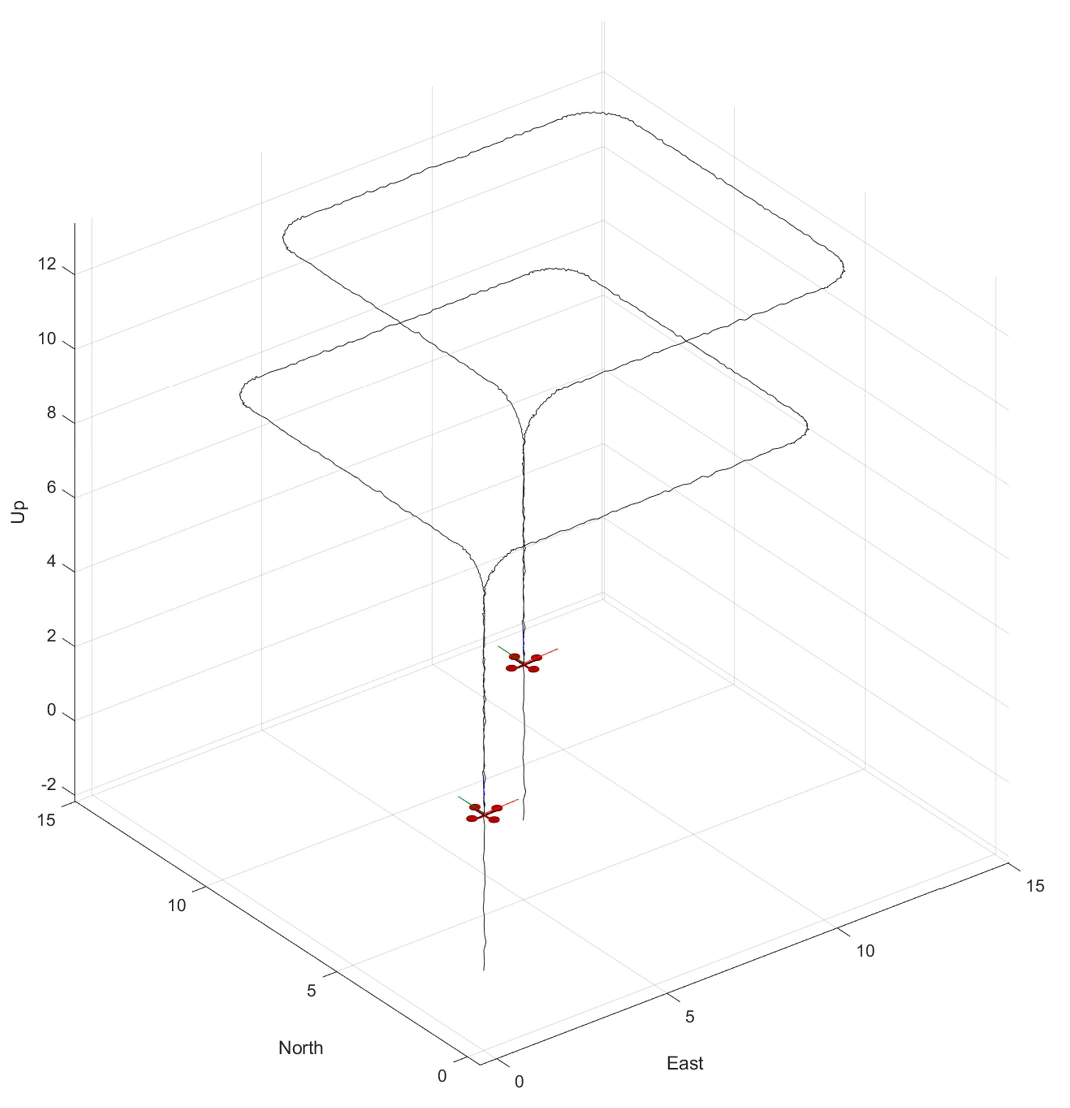
\includegraphics[width=\textwidth]{figs/Samuel/Figures/MultiAgentExampleRed (2).pdf}
        \caption{Multi-agent simulation demonstrating when drones are an unsafe distance apart (distances in metres).}
        \label{fig:1a}
    \end{subfigure}
    \hspace{0.01\textwidth}
    \begin{subfigure}[b]{0.48\textwidth} % Use [b] to align captions at the bottom
        \centering
        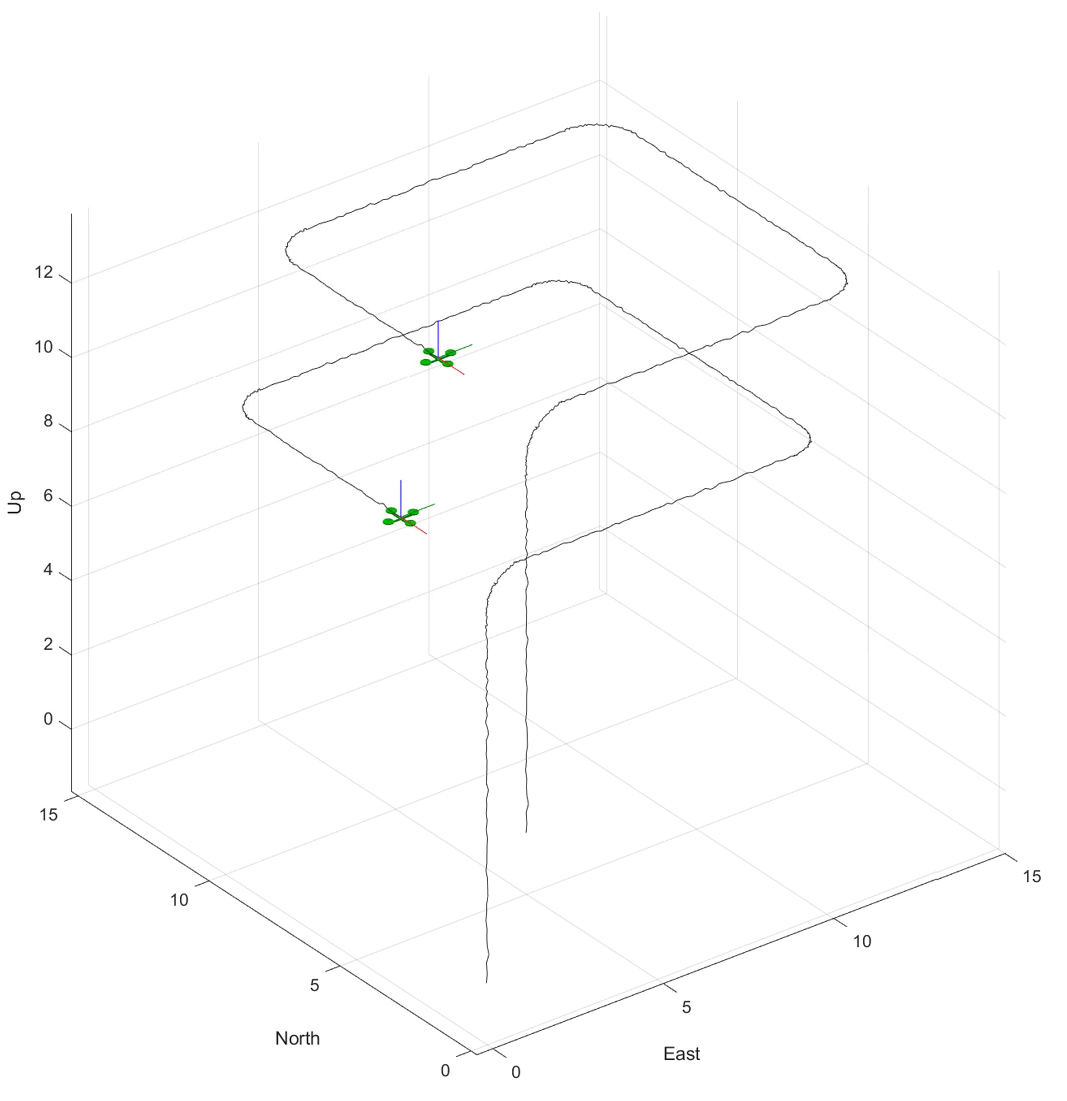
\includegraphics[width=\textwidth]{figs/Samuel/Figures/MultiAgentExampleGreen (2).pdf}
        \caption{Multi-agent simulation demonstrating when drones are a safe distance apart (distances in metres).}
        \label{fig:1b}
    \end{subfigure}
    \caption[Multi-agent Simulation]{Multi-agent simulation with drones an unsafe distance apart (a) and a safe distance apart (b).}
    \label{fig:dronemulti}
\end{figure}



\subsection{Wind Gust Mitigation}
\label{gust}
Modelling the effects of wind disturbances is crucial to assessing the viability of a mission. Within the range of acceptable wind speeds, the controller must be sufficiently robust to wind disturbances so that a steady hovering position can be maintained. This requirement is necessary because a key constraint on the drone's sensing capabilities is its ability to accurately maintain a set reference position. The approach taken uses an Application Programming Interface (API) to access current and future weather data for the specified coordinates of the drone's mission and then takes the maximum wind speed as an input to the simulation. 

The \href{https://www.meteomatics.com/}{\textbf{Meteomatics API}}  is used to find the u, v and w components\footnote{u and v measure wind speed from west to east and south to north respectively, and w measures downward wind speed \cite{meteomatics_wind_speed}} of the wind speed for a given location \cite{meteomatics_wind_speed}. Running these simulations allows a decision to be made in advance as to whether a mission is viable at a particular time. This avoids both unnecessary expense in travelling and setting up for an unfeasible mission and ensures the drone is not damaged due to being operated in hazardous conditions. While the \href{https://www.meteomatics.com/}{\textbf{Meteomatics API}}
provides a valuable forecast of the weather conditions, there is an inherent degree of uncertainty present due to the random nature of gusts of wind. To enhance the drone's ability to withstand sudden wind gusts, it is crucial to harness the power of artificial intelligence to compute \textbf{online estimates} of incoming gust occurrences. 

\subsubsection{Machine Learning Techniques}
\label{sec:mlalgos}

One of the key constraints on the drone's ability to gather reliable sensor data is how well it can tolerate sudden gusts of wind. Providing the drone with advance warning of when wind gusts are expected would significantly improve the drone's ability to remain stable at all times. The drone is equipped with various sensors, including a gyroscope and an accelerometer. Using the data from these sensors in combination with machine learning algorithms makes it possible to predict when the drone will experience a sudden gust of wind during flight.

To make the gust prediction, a \textbf{binary classifier} is required to decide whether the conditions indicate the presence or absence of an incoming gust. The dataset chosen to train the machine learning model is labelled, so a \textbf{supervised learning algorithm} is appropriate. The use of drone sensor data in predicting wind gusts has been attempted previously \cite{gu2018wind}. However, this approach will consider the application of additional algorithms which, to the best of the author's knowledge, have not been utilised in this context before. Although deep neural networks (DNN) have now become ubiquitous in the field of machine learning, the dataset being considered here contains too few data samples for DNNs to provide useful results \cite{golestaneh2024samplesneededtraindeep}. Instead, a simpler approach needs to be considered. 

The  \textbf{Synthetic Minority Oversampling Technique (SMOTE)} algorithm can be used to improve the performance of a classifier operating on an imbalanced dataset, by generating additional minority datapoints using interpolation \cite{chawla2002smote}. As is often the case, the real-world dataset for gust conditions contains many datapoints for the absence of a gust, but only a small percentage of the readings correspond to the \textit{interesting case} of the presence of a gust. The use of SMOTE allows for the dataset to be artificially rebalanced and has the potential to improve the performance of the binary classifier significantly.

In this instance, a basic implementation of the random forest classifier \cite{scikit-learn} is used in Python to classify the data. A labelled dataset is utilised from a previous implementation of drone gust detection \cite{gu2018wind}, and the data is preprocessed by introducing additive Gaussian noise (AGN) to simulate real-world sensor inaccuracies. The data is split using an \textbf{80/20 train-test split}, and the random forest model is then trained on the data. 

To perform a comparative evaluation on the effect of the number of trees used in the random forest, the F-2 score is used as the performance metric because it prioritises recall over precision. The model's F-2 score is evaluated while varying the number of trees used. Figure \ref{fig:radchart} shows the average variation of performance metrics (including the F-2 score) with an increasing number of trees. 

\subsubsection{Evaluation}

Figure \ref{fig:featureimportance} shows the normalised feature importance for each of the measurements used in the machine learning model. The most important feature is the \textbf{gyroscope z-axis measurement}. This result is expected since the measurement is directly proportional to the angular velocity in the x-y plane, and the drone will rotate about the z-axis when the wind exerts a lateral force. The \textbf{gyroscope x and y axes measurements} are the next most important features, which is to be expected since the wind will also cause the drone to tilt in the x-z and y-z planes. The \textbf{accelerometer measurements} are much less important, as they measure linear motion rather than rotational, and are more sensitive to high frequency noise than comparable gyroscopes \cite{CASSON2016175}. 

These results suggest that, by only using gyroscope measurements, an online estimate could be computed more efficiently with minimal accuracy loss. The utility of this approach would depend on the processing power available onboard the drone since, if this were severely limited, using a smaller set of features may be crucial in effectively applying the classifier. 

If processing power was less of a constraint, however, the advantage of utilising the additional features may outweigh the associated increase in computational cost. Verifying the applicability of this observation would require a physical implementation onboard a drone in a real-world environment.

\begin{figure}[H]
\centering
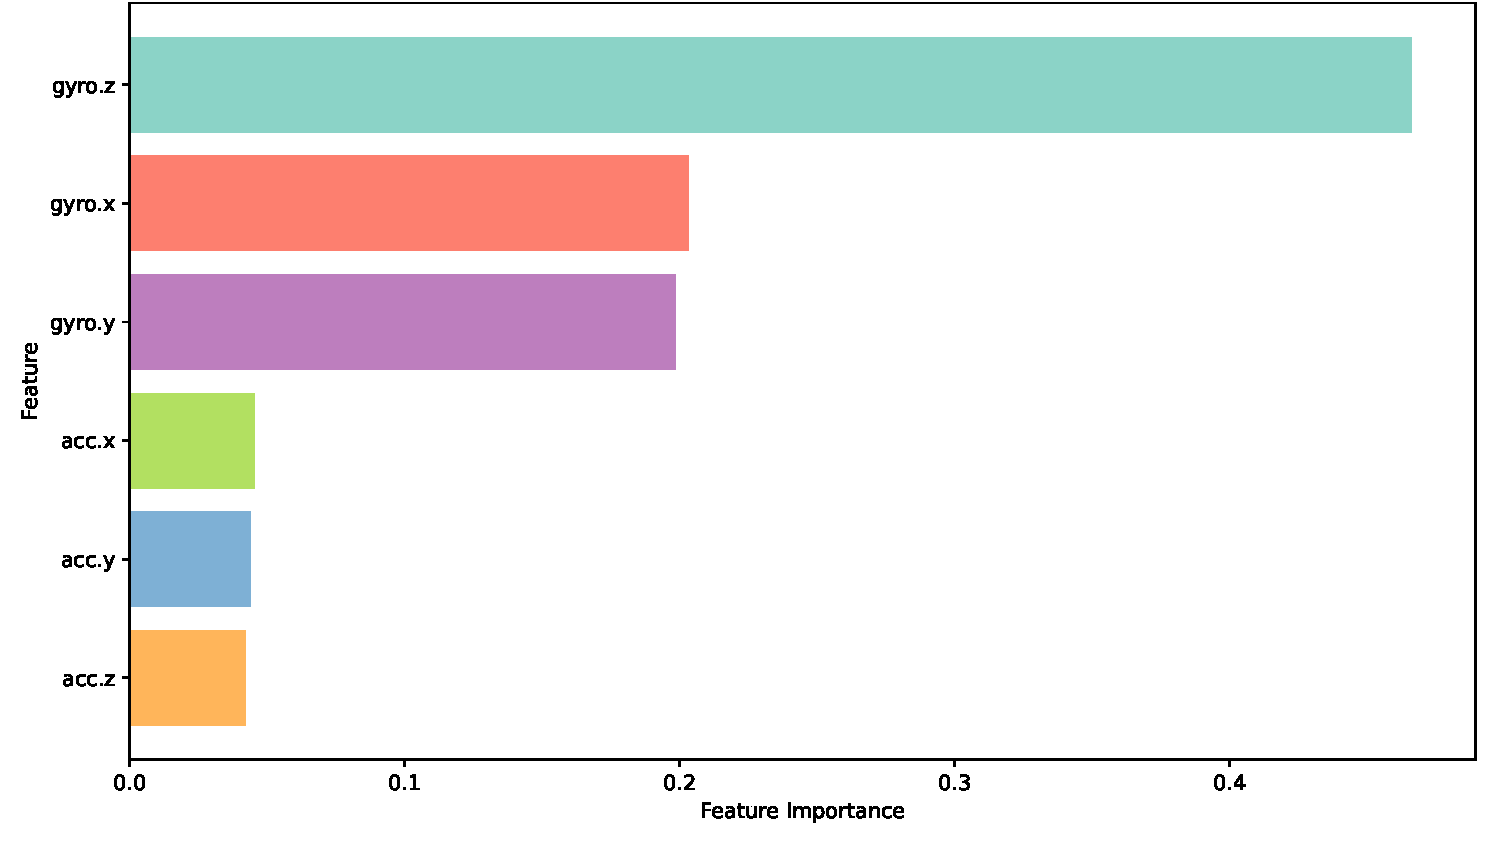
\includegraphics[width=0.70\textwidth]{figs/Samuel/Figures/feature_importance_smote (cropped) (pdfresizer.com).pdf}
\caption{Bar chart showing the normalised feature importance for the random forest classifier.}
\label{fig:featureimportance}
\end{figure}




Figure \ref{fig:radchart} shows how the random forest classifier performs depending on the number of decision trees used in the model. As expected, the addition of trees behaves as a law of diminishing returns, with the improvement from 10 to 50 trees being more noticeable than that from 50 to 100 trees. The model and data used to perform these predictions serve as a proof of concept, hence there is significant scope to improve the model and make it more robust to a wider range of sensor noise and uncertainties. The formulae for all of the performance metrics used on the diagram are given in Equations \ref{eq:precision} to \ref{eq:mcc}, where TP, TN, FP and FN represent true positives, true negatives, false positives and false negatives respectively.

\textbf{F-2 score} was selected instead of the more conventional F-1 score to place greater importance on recall rather than precision. The \gls{MCC} was also used due to its higher suitability for evaluating binary classifiers compared to the \gls{ROCAUC}. The benefits of the \acrshort{MCC} for binary classifier evaluation are discussed in \cite{Chicco2023}.

The model has a high average recall of approximately 0.8, when 50 or more decision trees are used. The F-2 score also approaches 0.8 when more than 50 trees are used. These results suggest that the model is performing as anticipated and effectively detects the majority of gusts, even if it occasionally flags false positives. To achieve further improvements, the model would likely require a larger dataset or the use of deep neural networks, as discussed in Section \ref{sec:modelfree}.



\vspace{10mm}


\noindent
\begin{minipage}{0.45\textwidth}
  \begin{equation}
    \text{Precision} = \frac{\text{TP}}{\text{TP} + \text{FP}}
    \label{eq:precision}
  \end{equation}
\end{minipage}
\hfill
\begin{minipage}{0.45\textwidth}
  \begin{equation}
    \text{Recall} = \frac{\text{TP}}{\text{TP} + \text{FN}}
  \end{equation}
\end{minipage}

\vspace{1mm}

\noindent
\begin{minipage}{0.45\textwidth}
  \begin{equation}
    \text{F-2}\text{ Score} = \frac{\text{5} \cdot \text{Precision} \cdot \text{Recall}}{\text{4} \cdot \text{Precision} + \text{Recall}}
  \end{equation}
\end{minipage}
\hfill
\begin{minipage}{0.45\textwidth}
\vspace{7mm}
  \begin{equation}
    \text{Accuracy} = \frac{\text{TP} + \text{TN}}{\text{TP} + \text{FP} + \text{TN} + \text{FN}}
  \end{equation}
\end{minipage}

\vspace{7mm}

\begin{equation}
\text{MCC} = \frac{ \text{TP} \cdot \text{TN} - \text{FP} \cdot \text{FN} }{ \sqrt{ (\text{TP} + \text{FP}) (\text{TP} + \text{FN}) (\text{TN} + \text{FP}) (\text{TN} + \text{FN}) } }
\label{eq:mcc}
\end{equation}









\begin{figure}[H]
\centering
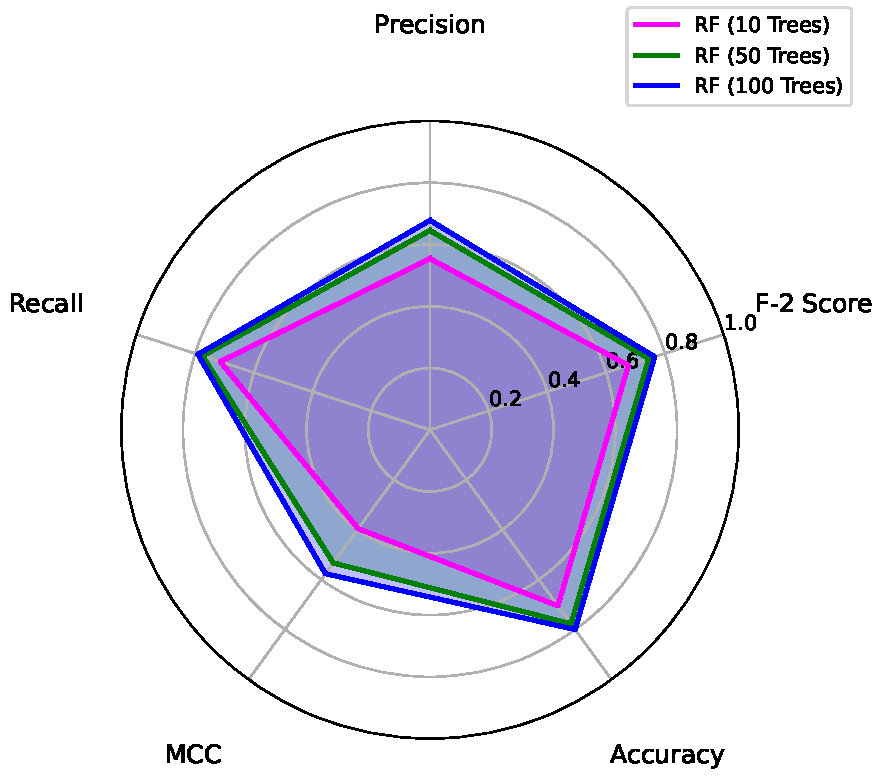
\includegraphics[width=0.74\textwidth]{figs/Samuel/Figures/rf_comparison (4) (1) (1).pdf}
\caption[Radar chart showing the performance of the random forest model]{Radar chart showing the variation of the model performance with a changing number of trees.}
\label{fig:radchart}
\end{figure}






\subsection{Embedded Algorithms}

The simulations performed in previous sections help build confidence as to whether strategies are viable, but the methods chosen must still be implemented onboard the drone. There are numerous options for implementing processes on a drone, with the most common and well-documented being the use of embedded C code on a microcontroller. For these reasons, all of the processes carried out onboard the drone are implemented using embedded C code. The algorithms are tested using the ARM GNU Toolchain in order to verify their suitability prior to deployment.

\subsubsection{\gls{BMS} Algorithms}

The algorithms required to implement the \gls{BMS} are run onboard an \textbf{STM32F405} microcontroller, with the MATLAB Coder used to convert all of the required processes into embedded C code. The Coder is configured to optimise the converted algorithms for the \textbf{STM32F405} because it is specified as the \textit{target hardware}. The exceptions to this method are the Kalman filtering algorithms, which utilise a pre-optimised C library, as discussed in Section \ref{kalm}. 

\subsubsection{Cascade \gls{PID} Control}

The cascade \gls{PID} control system is implemented onboard the drone using a controller which has been specifically designed in C for the STM32H7 board.\footnote{\url{https://github.com/ChrisWonyeobPark/PID-Control}} The lightweight implementation allows for the controller to have a high bandwidth, enabling it to respond quickly to any disturbances and rapidly return the drone to stability.

\subsubsection{Machine Learning Software}

Although the model used as a proof of concept in Section \ref{sec:mlalgos} was implemented using Python, future implementations could be trained using fast, lightweight random forest software in C++. The Random Forest C++ implementation by Bjoern Andres\footnote{\url{https://github.com/bjoern-andres/random-forest}} was selected for further analysis here. 

A \gls{UML} class diagram summarising the implementation is shown in Figure \ref{fig:uml}, with the attributes of the classes omitted for brevity. The model would then be implemented by using an existing C library for random forests, allowing its implementation onboard the drone for online gust predictions.\footnote{\url{https://github.com/andriidski/random-forests-c/tree/master}} The separation of the training and implementation software ensures that the hyperparameters are sufficiently optimised without requiring excessive processing power onboard the drone.

\begin{figure}[H]
\centering
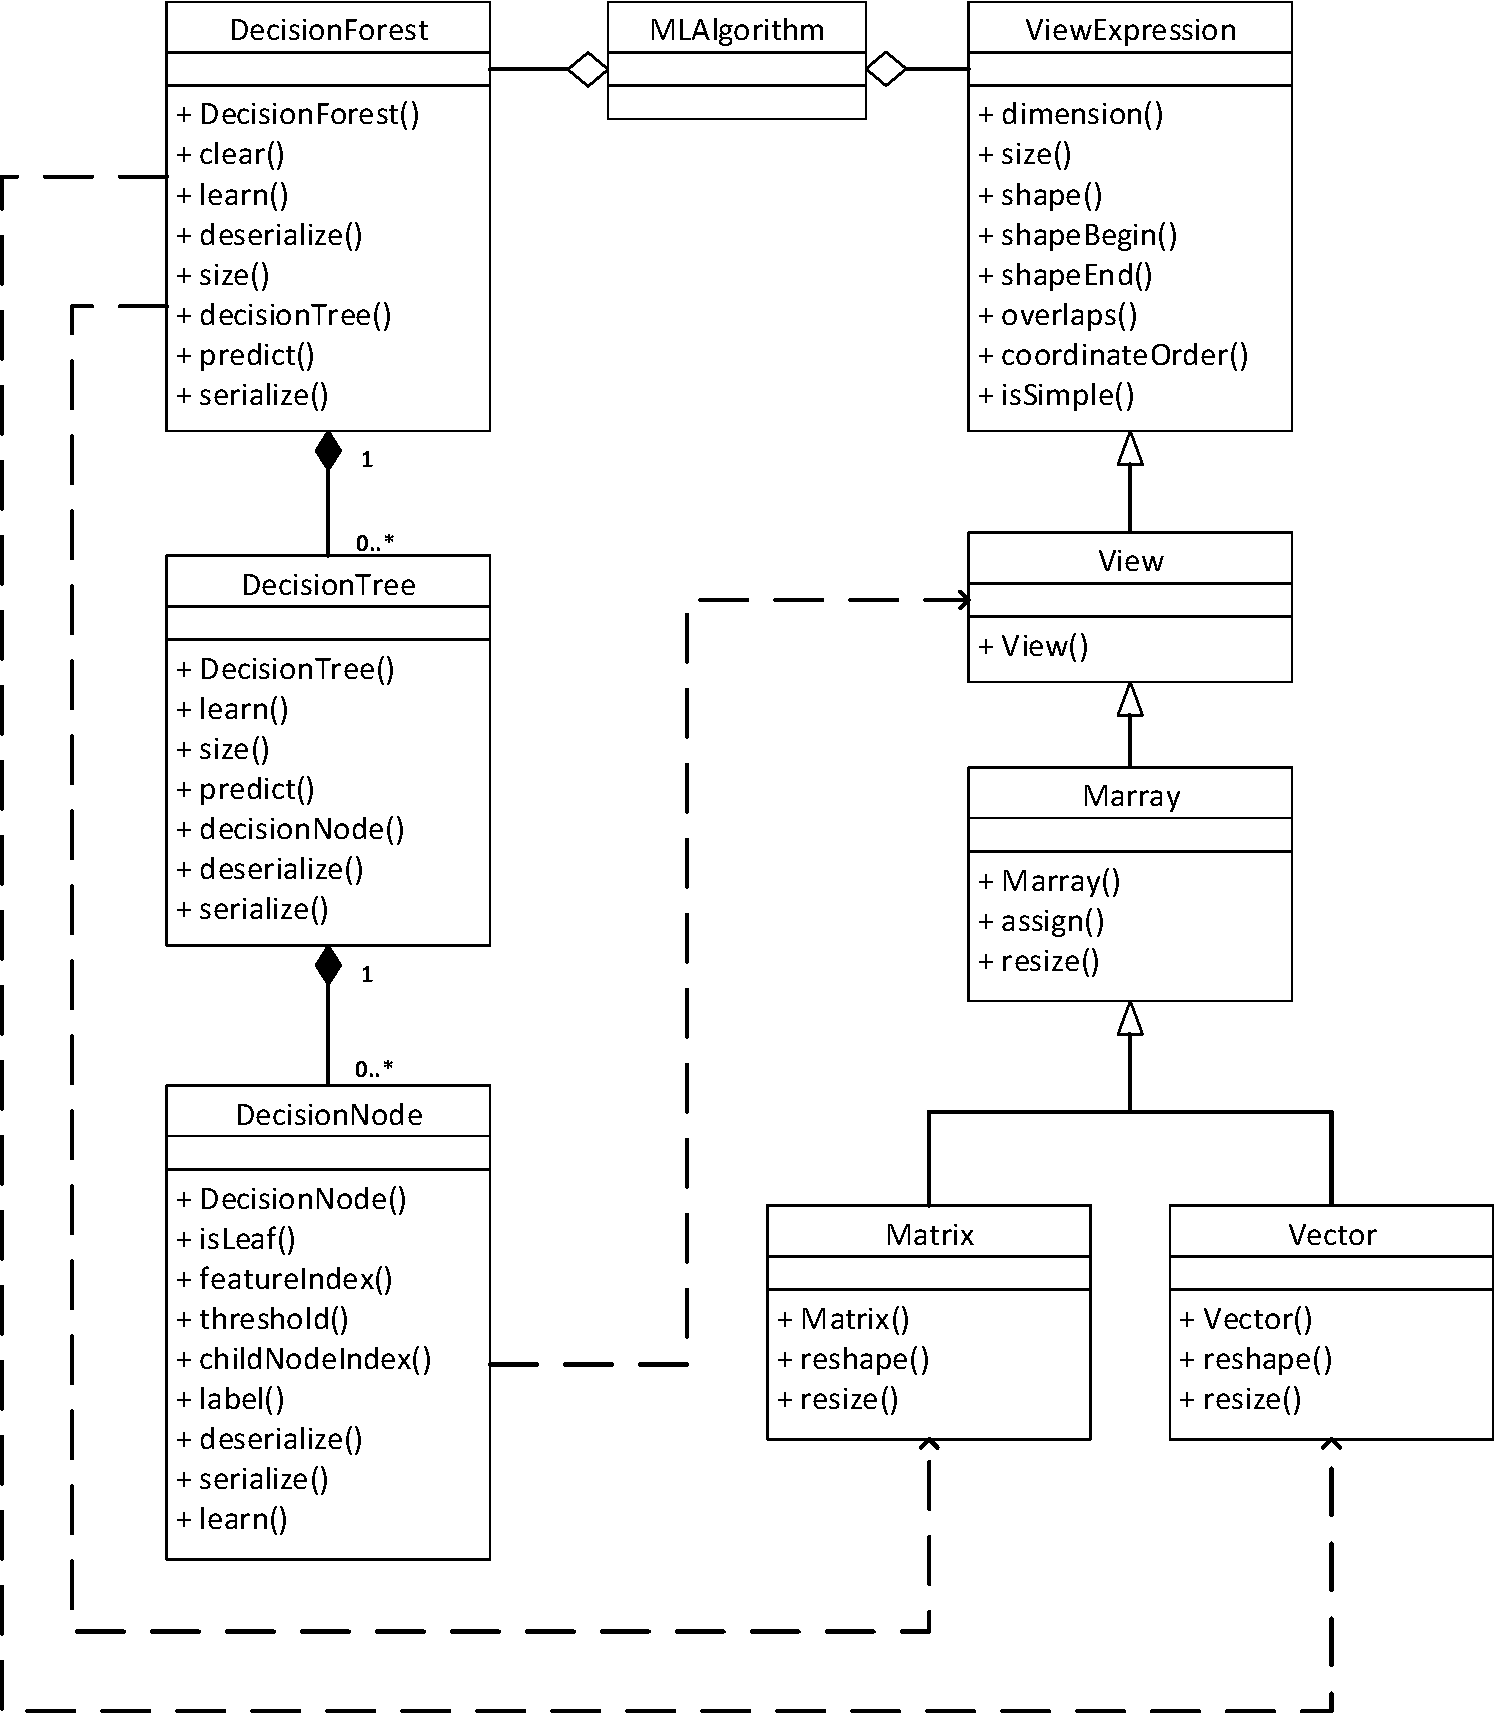
\includegraphics[width=0.99\textwidth]{figs/Samuel/Figures/UML Random Forest-cropped.pdf}
\caption{UML Class Diagram for Bjoern Andres' Random Forest C++ implementation.}
\label{fig:uml}
\end{figure}




\subsection{Conclusion and Ideas for Future Work}

\subsubsection{Control Techniques}
\label{sec:modelfree}

The appeal of the cascade \gls{PID} control strategy is its simplicity and ease of modification. However, ongoing developments in microcontroller processing power will be advantageous and allow for more sophisticated methods to be implemented onboard the drone.

The first potential improvement could be made by combining the \gls{LQR} and \gls{PID} control techniques onboard the drone, so that the drone can benefit from the robustness of the \gls{PID} controller in general flight, while being able to hover more steadily using a finely tuned \gls{LQR}. Model predictive control (\acrshort{MPC}) could also be investigated to allow the drone's controller to be updated during the mission, although this method would require a significant increase in onboard processing power. 

Backstepping could also be investigated, which involves dividing the system into smaller subsystems and designing the overall control scheme recursively, allowing the full nonlinear system to be modelled while ensuring that Lyapunov stability is satisfied \cite{4058900}. 

Innovative machine learning techniques offer the possibility of designing model-free controllers. The use of this strategy would allow for the controller's performance to be further improved. All of these techniques have the potential to improve the flight controller's performance but introduce additional complexity and cost to the theoretical model and the embedded code.

\subsubsection{Machine Learning for Wind Gust Detection}

The machine learning model discussed in this report serves as a proof of concept for online gust detection; the limited size of the dataset available acted as a constraint on the models that could be employed. Deploying the model onboard a drone to evaluate its effectiveness and gathering a larger labelled dataset would be required to further develop this idea. 

Significant improvements would likely be achievable if a sufficiently large dataset was used to train a \gls{DNN}. Alternatively, the problem could be recast as a \textbf{regression} problem, where the model predicts the speed of the incoming gust rather than simply its occurrence. Solving this problem would again require a significantly larger dataset, but would provide more informative predictions by allowing the drone to gradually increase the power boost to the rotors depending on gust intensity.



